%%%% comparacao_workflows.tex
%%%% Comparação do fluxo de trabalho com agentes de IA nas quatro tentativas do projeto AIS.
%%%% REV-084 (cor Azul-aço-escuro #1F4E79): documento novo. REV-085 (Cinzento-grafite #3C3C3C):
%%%% a pedido do utilizador, todo o texto passa a preto; a cor fica só nas molduras das caixas.
%%%% Compilar a partir de investigacao_agentes/:  pdflatex comparacao_workflows.tex (duas vezes).
%%%% Os números vêm de gerado/metricas.tex, gerado por scripts/metricas_git.py (não editar à mão).

\documentclass[11pt,a4paper]{article}
\usepackage[utf8]{inputenc}
\usepackage[T1]{fontenc}
\usepackage{lmodern}
\usepackage{textcomp}
\DeclareUnicodeCharacter{2248}{\ensuremath{\approx}}
\usepackage[provide=*,portuguese]{babel}
\usepackage[a4paper,margin=2.3cm]{geometry}
\usepackage{xcolor}
\usepackage{graphicx}
\usepackage{booktabs}
\usepackage{tabularx}
\usepackage{array}
\usepackage{enumitem}
\usepackage[most]{tcolorbox}
\usepackage{listings}
\usepackage{caption}
\usepackage{float}
\usepackage[hidelinks]{hyperref}
\usepackage{microtype}

% Revisões (AGENTS.md §8): mesma cor do REVISION_LOG.md.
\definecolor{rev084}{HTML}{1F4E79}
\newcommand{\revtext}[2]{{\color{#1}#2}}

% Gerado por investigacao_agentes/scripts/metricas_git.py (REV-084). Não editar.
\newcommand{\mUmCommits}{41}
\newcommand{\mUmDias}{11}
\newcommand{\mUmBranches}{3}
\newcommand{\mUmPrimeiro}{02/10/2026}
\newcommand{\mUmUltimo}{26/11/2026}
\newcommand{\mUmFicheiros}{69}
\newcommand{\mUmLinhasPy}{1053}
\newcommand{\mUmLinhasTestes}{283}
\newcommand{\mUmFuncTestes}{14}
\newcommand{\mUmLinhasMd}{2526}
\newcommand{\mUmRegisto}{2}
\newcommand{\mUmComRev}{0}
\newcommand{\mUmAgentsVersoes}{2}
\newcommand{\mUmAgentsLinhas}{81}
\newcommand{\mUmCoAutor}{9}
\newcommand{\mUmCoAutorCopilot}{9}
\newcommand{\mUmCoAutorHaiku}{0}
\newcommand{\mUmCoAutorSonnet}{0}
\newcommand{\mUmCoAutorOpus}{0}
\newcommand{\mUmSoMd}{3}
\newcommand{\mUmAgentsPrimeiro}{32}
\newcommand{\mDoisCommits}{39}
\newcommand{\mDoisDias}{3}
\newcommand{\mDoisBranches}{4}
\newcommand{\mDoisPrimeiro}{16/11/2026}
\newcommand{\mDoisUltimo}{20/11/2026}
\newcommand{\mDoisFicheiros}{77}
\newcommand{\mDoisLinhasPy}{1447}
\newcommand{\mDoisLinhasTestes}{0}
\newcommand{\mDoisFuncTestes}{0}
\newcommand{\mDoisLinhasMd}{2694}
\newcommand{\mDoisRegisto}{0}
\newcommand{\mDoisComRev}{0}
\newcommand{\mDoisAgentsVersoes}{5}
\newcommand{\mDoisAgentsLinhas}{56}
\newcommand{\mDoisCoAutor}{0}
\newcommand{\mDoisCoAutorCopilot}{0}
\newcommand{\mDoisCoAutorHaiku}{0}
\newcommand{\mDoisCoAutorSonnet}{0}
\newcommand{\mDoisCoAutorOpus}{0}
\newcommand{\mDoisSoMd}{8}
\newcommand{\mDoisAgentsPrimeiro}{32}
\newcommand{\mTresCommits}{14}
\newcommand{\mTresDias}{3}
\newcommand{\mTresBranches}{1}
\newcommand{\mTresPrimeiro}{20/11/2026}
\newcommand{\mTresUltimo}{26/11/2026}
\newcommand{\mTresFicheiros}{27}
\newcommand{\mTresLinhasPy}{3854}
\newcommand{\mTresLinhasTestes}{0}
\newcommand{\mTresFuncTestes}{0}
\newcommand{\mTresLinhasMd}{471}
\newcommand{\mTresRegisto}{1}
\newcommand{\mTresComRev}{0}
\newcommand{\mTresAgentsVersoes}{4}
\newcommand{\mTresAgentsLinhas}{145}
\newcommand{\mTresCoAutor}{1}
\newcommand{\mTresCoAutorCopilot}{1}
\newcommand{\mTresCoAutorHaiku}{0}
\newcommand{\mTresCoAutorSonnet}{0}
\newcommand{\mTresCoAutorOpus}{0}
\newcommand{\mTresSoMd}{1}
\newcommand{\mTresAgentsPrimeiro}{121}
\newcommand{\mQuatroCommits}{150}
\newcommand{\mQuatroDias}{4}
\newcommand{\mQuatroBranches}{1}
\newcommand{\mQuatroPrimeiro}{23/11/2026}
\newcommand{\mQuatroUltimo}{26/11/2026}
\newcommand{\mQuatroFicheiros}{177}
\newcommand{\mQuatroLinhasPy}{7003}
\newcommand{\mQuatroLinhasTestes}{3343}
\newcommand{\mQuatroFuncTestes}{209}
\newcommand{\mQuatroLinhasMd}{4249}
\newcommand{\mQuatroRegisto}{38}
\newcommand{\mQuatroComRev}{131}
\newcommand{\mQuatroAgentsVersoes}{21}
\newcommand{\mQuatroAgentsLinhas}{270}
\newcommand{\mQuatroCoAutor}{150}
\newcommand{\mQuatroCoAutorCopilot}{0}
\newcommand{\mQuatroCoAutorHaiku}{31}
\newcommand{\mQuatroCoAutorSonnet}{100}
\newcommand{\mQuatroCoAutorOpus}{19}
\newcommand{\mQuatroSoMd}{68}
\newcommand{\mQuatroAgentsPrimeiro}{259}


\setlist{itemsep=2pt,topsep=4pt}
\captionsetup{font=small,labelfont=bf}
\renewcommand{\arraystretch}{1.15}
\newcolumntype{L}{>{\raggedright\arraybackslash}X}

\newcommand{\facto}{\textsc{[facto]}}
\newcommand{\deducao}{\textsc{[dedução]}}
\newcommand{\Pum}{\textbf{P1}}
\newcommand{\Pdois}{\textbf{P2}}
\newcommand{\Ptres}{\textbf{P3}}
\newcommand{\Pquatro}{\textbf{P4}}

\newtcolorbox{sintese}[1][]{colback=rev084!5,colframe=rev084!70,fonttitle=\bfseries,
  title={#1},boxrule=0.6pt,arc=2pt,left=6pt,right=6pt,top=4pt,bottom=4pt}
\newtcolorbox{licao}[1][]{colback=white,colframe=rev084,fonttitle=\bfseries,
  title={#1},boxrule=0.8pt,arc=2pt,left=6pt,right=6pt,top=4pt,bottom=4pt}

\lstset{basicstyle=\ttfamily\footnotesize,breaklines=true,columns=fullflexible,
  frame=single,rulecolor=\color{rev084!40},backgroundcolor=\color{rev084!3},
  extendedchars=true,keepspaces=true,
  literate={á}{{\'a}}1 {à}{{\`a}}1 {â}{{\^a}}1 {ã}{{\~a}}1 {ç}{{\c{c}}}1 {é}{{\'e}}1
   {ê}{{\^e}}1 {í}{{\'i}}1 {ó}{{\'o}}1 {õ}{{\~o}}1 {ú}{{\'u}}1 {Ú}{{\'U}}1
   {«}{{\guillemotleft}}1 {»}{{\guillemotright}}1 {→}{{$\rightarrow$}}1 {≈}{{$\approx$}}1
   {–}{{--}}1 {—}{{---}}1}

\title{\textbf{Do caos ao fluxo}\\[4pt]
\large Comparação do fluxo de trabalho com agentes de IA\\ nas quatro tentativas do projeto AIS}
\author{Dinis Rosa\\[2pt]\small Universidade de Coimbra, Departamento de Engenharia Informática}
\date{26 de novembro de 2026}

\begin{document}
\maketitle

\begin{abstract}
\noindent Este documento analisa como foi feito, com agentes de IA, um projeto universitário de
segmentação de viagens AIS em pesca e navegação. O projeto teve quatro tentativas, cada uma num
repositório GitHub próprio (\Pum{} a \Pquatro). Entre tentativas mudou sobretudo o \emph{fluxo de
trabalho}: os documentos de instrução dados ao agente, as regras, a forma de comunicar e os
mecanismos para guardar estado e raciocínio entre sessões. Os quatro históricos git foram lidos
por quatro subagentes (um por repositório) e as métricas foram calculadas por um script
versionado. A conclusão principal é que a tentativa que terminou (\Pquatro, com Claude Code) não
se distingue por ter mais regras, mas por ter as regras \emph{certas desde o primeiro commit}:
marcos executáveis, isolamento auditável dos dados reservados, números gerados por código,
testes sintéticos e um ficheiro de passagem de testemunho entre sessões. Os principais problemas
que persistiram foram o excesso de exploração e de contabilidade face ao progresso real
(«muito por pouco»). O documento termina com um kit de arranque para projetos futuros.

\medskip
\noindent\textbf{Abstract.} This report compares the AI-agent workflow across four attempts of a
university project on AIS trajectory segmentation. The finished attempt (P4, Claude Code) did not
win by having more rules, but by having the right ones from the first commit: executable
milestones, auditable isolation of held-out data, code-generated numbers, synthetic tests and a
session handoff file. Over-exploration and bookkeeping overhead persisted. A reusable starter kit
is provided.
\end{abstract}

\tableofcontents
\newpage

%% =====================================================================
\section{Introdução}

O projeto da unidade curricular IACH pedia a segmentação semântica de trajetórias AIS (o sinal de
posição dos navios) para detetar atividade de pesca, com uma previsão por ponto e uma CNN~1D como
modelo principal. O trabalho foi feito «maioritariamente por mim com a ajuda de um agente, neste
caso vários agentes». Houve quatro tentativas, cada uma num repositório público próprio:

\begin{center}\small
\begin{tabularx}{\linewidth}{@{}lL@{}}
\toprule
\Pum & \url{https://github.com/DinisRosa/IACH-AIS-Project}\\
\Pdois & \url{https://github.com/DinisRosa/IACH-AIS-Project_2}\\
\Ptres & \url{https://github.com/DinisRosa/IACH-AIS-Project_3}\\
\Pquatro & \url{https://github.com/DinisRosa/IACH-AIS-Project_4} (onde está este documento)\\
\bottomrule
\end{tabularx}
\end{center}

Em cada tentativa o código mudou, mas a mudança mais deliberada foi no \emph{fluxo de trabalho}
entre o utilizador e o agente (o \emph{agentic flow}): que documentos se enviavam, como se
enviavam, que regras se criavam e como se guardava o raciocínio e o estado entre sessões.
Este documento responde a cinco perguntas:

\begin{enumerate}[label=\textbf{Q\arabic*}]
  \item Como foi feito cada projeto e como comunicavam o utilizador e o agente?
  \item Como se manteve a segurança (dados reservados, git, permissões)?
  \item Como se manteve a fiabilidade (testes, reprodutibilidade, verdade sobre o que foi feito)?
  \item O que correu bem e o que correu mal, no início e ainda agora?
  \item O que fazer no próximo projeto para começar logo a trabalhar bem?
\end{enumerate}

O documento destina-se ao autor, ao docente e a qualquer pessoa que trabalhe com agentes de
programação. A Secção~\ref{sec:metodo} descreve o método; a Secção~\ref{sec:tentativas}, cada
tentativa; a Secção~\ref{sec:comparacao} compara-as por eixos; as Secções~\ref{sec:balanco}
e~\ref{sec:licoes} fazem o balanço e tiram lições; a Secção~\ref{sec:kit} apresenta o kit de
arranque, cujos modelos estão nos anexos e em \texttt{investigacao\_agentes/kit/}.

%% =====================================================================
\section{Método}\label{sec:metodo}

\paragraph{Fontes.} Por decisão do utilizador, só se usaram os quatro repositórios GitHub, com o
histórico completo de todas as branches. Não se leram conversas, pastas locais nem outros
projetos. Os repositórios foram clonados em modo só de leitura para uma pasta temporária,
apagada no fim; nenhum foi alterado. Não se abriram ficheiros de dados AIS.

\paragraph{Análise.} Quatro subagentes (modelo Claude Opus), um por repositório, estudaram o
histórico com comandos git de leitura e responderam às mesmas dez perguntas: cronologia,
ferramenta usada, documentos de instrução, memória, segurança, fiabilidade, produtividade,
estrutura, o que correu bem e mal, e traços distintivos. Cada afirmação foi marcada como
\facto{} (com commit, data ou caminho) ou \deducao{} (inferência). O coordenador integrou os
relatórios, verificou por amostragem as afirmações centrais e escreveu este documento.

\paragraph{Números.} Os números das tabelas e figuras vêm do script
\texttt{scripts/metricas\_git.py} (na pasta \texttt{investigacao\_agentes/}), que lê os clones e grava
\texttt{gerado/metricas.json}, \texttt{gerado/metricas.tex} e as figuras. Segue a regra de
reprodutibilidade do próprio \Pquatro{} (AGENTS.md §10). Commits contam-se em todas as branches;
linhas de código e testes contam-se na branch por defeito. Alguns números pontuais (por exemplo,
linhas de um ficheiro concreto) vêm dos relatórios dos subagentes e indicam o commit de origem.

\paragraph{Ferramentas.} O utilizador usou opencode, Cline, Abacus.AI, GitHub Copilot e
Antigravity (Gemini) nas três primeiras tentativas, e Claude Code na quarta, mas não se lembrava
qual em qual. A atribuição por tentativa é por isso uma \deducao{}, baseada em vestígios no
repositório (ficheiros-ponte, entradas no \texttt{.gitignore}, \emph{trailers}
\texttt{Co-authored-by} e texto dos documentos).

\paragraph{Limitações.} As conversas com os agentes não estão versionadas; muito do que o
utilizador pediu só se vê indiretamente. Em \Pum{} a pasta \texttt{docs/} esteve fora do git
durante cerca de cinco semanas. Contar linhas ou commits mede esforço visível, não valor.
Ver Secção~\ref{sec:validade}.

\begin{table}[H]
\centering\small
\caption{Visão geral das quatro tentativas (métricas geradas por \texttt{metricas\_git.py}).}
\label{tab:visao}
\begin{tabularx}{\linewidth}{@{}>{\raggedright\arraybackslash}p{3.2cm}LLLL@{}}
\toprule
 & \Pum & \Pdois & \Ptres & \Pquatro \\
\midrule
Período & \mUmPrimeiro{} a \mUmUltimo & \mDoisPrimeiro{} a \mDoisUltimo & \mTresPrimeiro{} a \mTresUltimo & \mQuatroPrimeiro{} a \mQuatroUltimo \\
Commits (dias ativos) & \mUmCommits{} (\mUmDias) & \mDoisCommits{} (\mDoisDias) & \mTresCommits{} (\mTresDias) & \mQuatroCommits{} (\mQuatroDias) \\
Branches & \mUmBranches & \mDoisBranches & \mTresBranches & \mQuatroBranches \\
Ferramenta (dedução) & Copilot, opencode, Abacus.AI & opencode; outro agente no fim & Copilot ou Cline & Claude Code \\
Linhas Python / testes & \mUmLinhasPy{} / \mUmLinhasTestes & \mDoisLinhasPy{} / \mDoisLinhasTestes & \mTresLinhasPy{} / \mTresLinhasTestes & \mQuatroLinhasPy{} / \mQuatroLinhasTestes \\
Funções de teste & \mUmFuncTestes & \mDoisFuncTestes & \mTresFuncTestes{} (asserts nos scripts) & \mQuatroFuncTestes{} (256 casos) \\
AGENTS.md (linhas, versões) & \mUmAgentsLinhas{}, \mUmAgentsVersoes & \mDoisAgentsLinhas{}, \mDoisAgentsVersoes & \mTresAgentsLinhas{}, \mTresAgentsVersoes & \mQuatroAgentsLinhas{}, \mQuatroAgentsVersoes \\
Até onde chegou & EDA e divisão; sem modelo & janelas e Dataset; modelo não treinado & BiGRU treinada; teste por fazer & tudo, com relatório \\
\bottomrule
\end{tabularx}
\end{table}

\begin{figure}[H]
\centering
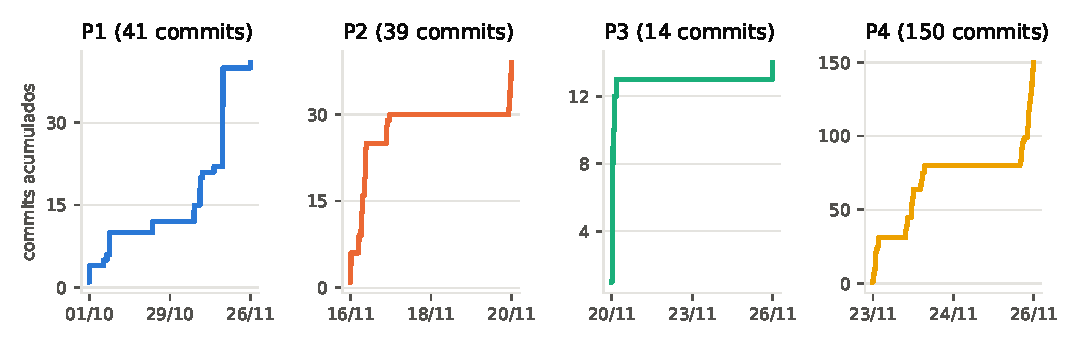
\includegraphics[width=\linewidth]{gerado/fig_commits_acumulados.pdf}
\caption{Commits acumulados ao longo do tempo em cada tentativa (todas as branches; escalas
diferentes). \Pum{} arrastou-se por oito semanas; \Pquatro{} concentrou 150 commits em quatro
dias, com uma pausa de cerca de 42~h a meio.}
\label{fig:commits}
\end{figure}

%% =====================================================================
\section{As quatro tentativas}\label{sec:tentativas}

\subsection{\Pum{} — muitas ferramentas, regras tardias, nenhum modelo}

\paragraph{Cronologia.} \facto{} \mUmCommits{} commits entre \mUmPrimeiro{} e \mUmUltimo{}, em
três branches (\texttt{main}, \texttt{features\_engineering}, \texttt{model\_training}). As
primeiras semanas foram a proposta em LaTeX e a bibliografia; seguiram-se ferramentas de dados e
análise exploratória (EDA); a 16 de novembro houve 18 commits num só dia, quase todos de
reorganização do repositório (nova raiz, \texttt{git subtree}, arquivo de dados, ramos de fase).
O ramo \texttt{model\_training} tem uma árvore idêntica à de \texttt{main}.

\paragraph{Ferramentas.} \facto{} \mUmCoAutorCopilot{} commits têm o \emph{trailer}
\texttt{Co-authored-by: Copilot}; o \texttt{.gitignore} passou a ignorar \texttt{.opencode/}
(commit \texttt{afff28c}) e \texttt{.abacusai/} (\texttt{6e8beb9}); o commit \texttt{de4c55f}
versionou cinco \emph{skills} do pacote \emph{superpowers} (brainstorming, writing-plans,
executing-plans, \dots) e uma skill própria, \texttt{delegate-terminal}, que delegava trabalho na
Abacus.AI ou no opencode «para poupar a quota do modelo principal». \deducao{} Copilot e opencode
com confiança alta; Abacus.AI como executor delegado; sem vestígios de Cline nem Antigravity.

\paragraph{Instruções e comunicação.} \facto{} O \texttt{AGENTS.md} só nasceu a 16 de novembro,
como subproduto da reorganização, e tratava quase só de git (ramo por fase, nunca
\emph{force-push}, evitar \texttt{git add .}). Não tinha regras de método, de âmbito, de dados
nem de comunicação. Antes disso, a comunicação fazia-se pela própria proposta e por três
revisões dela (uma com 1\,243 linhas) e, a partir de 13 de novembro, por pares
\emph{spec}/\emph{plan} muito prescritivos (um plano de 207 linhas para um conversor de 170).
A pasta \texttt{docs/} foi deixada de versionar a 8 de outubro (\texttt{a3ec4af}), pelo que o
raciocínio dessas semanas não sobreviveu no repositório.

\paragraph{Memória.} \facto{} Não havia registo de progresso nem de decisões. As 78
\emph{checkboxes} dos quatro planos ficaram todas por marcar, embora pelo menos três planos
tenham sido executados; o plano do \emph{baseline} nunca foi implementado e não deixou registo
de abandono.

\paragraph{Segurança.} \facto{} A proposta inicial dividia os dados por navio, «para evitar fuga
de informação»; a \emph{spec} de 13 de novembro passou a divisão por ID de viagem, aceitando que
viagens do mesmo navio caíssem em conjuntos diferentes. A EDA e a figura de normalização foram
calculadas sobre o conjunto completo, antes da divisão. Um CSV de 10~MB esteve no histórico, e os
conjuntos de treino, teste e validação derivados foram versionados num arquivo partido em três
partes de 90~MiB (cerca de 202~MB) no ramo \texttt{features\_engineering}. Um ficheiro de
constantes tinha caminhos absolutos da máquina pessoal.

\paragraph{Fiabilidade.} \facto{} \mUmFuncTestes{} testes pytest, só sobre o conversor e a
divisão (bons: dados sintéticos, sem escrever ficheiros reais). Sem \texttt{requirements.txt}.
Dois conversores concorrentes escreviam no mesmo ficheiro com esquemas diferentes, e o oficial
partia a EDA.

\paragraph{Produtividade.} \facto{} Cerca de 48\,\% das linhas de Python serviam para produzir
figuras (639 de 1\,336); 18 PNG no ramo de fase; nenhuma linha com \texttt{torch},
\texttt{keras} ou \texttt{sklearn}. O dia mais ativo produziu zero linhas de modelo.

\begin{sintese}[Em síntese — \Pum]
É o retrato exato da queixa «faziam muito por pouco»: muita estatística, muitas figuras, muitas
revisões e muita engenharia de git, e o modelo nunca começou. As instruções ao agente chegaram
tarde e só falavam de git. Várias ferramentas em paralelo, sem um registo comum, e a estrutura
mudou de raiz duas vezes. O utilizador recomeçou porque o repositório ficou caótico.
\end{sintese}

\subsection{\Pdois{} — um só ramo útil, planos externos e auditorias}

\paragraph{Cronologia.} \facto{} \mDoisCommits{} commits entre \mDoisPrimeiro{} e
\mDoisUltimo{}, em \mDoisDias{} dias com commits, dos quais 17 numa só noite (23:48--02:56).
Os ramos \texttt{code} e \texttt{latex} começaram como «um por área» e acabaram como
\emph{snapshots} de segurança nunca integrados, que ficaram obsoletos 13 horas depois. O trabalho
real foi linear em \texttt{main}.

\paragraph{Ferramentas.} \facto{} Nenhum ficheiro-ponte; só um \texttt{AGENTS.md} genérico. A
auditoria de 17 de novembro executou um notebook para \texttt{/tmp/opencode/\dots}.
\deducao{} opencode com confiança alta na fase intensa; a 20 de novembro, os assuntos sem
acentos e o vocabulário brasileiro sugerem outro agente ou modelo (Copilot, Cline ou o próprio
opencode; não se distingue).

\paragraph{Instruções e comunicação.} \facto{} O primeiro \texttt{AGENTS.md} (32 linhas) é uma
cópia exata de uma versão \emph{antiga} do de \Pum{}, com ramos e pastas que não existiam em
\Pdois; o agente trabalhou cerca de 6~h30 com instruções desatualizadas até à reescrita
(\texttt{7b4e193}). Regras acrescentadas depois de problemas: a de mensagens de commit
(\texttt{b6f7ab6}) surge 4 minutos depois de um commit sem corpo que misturava janelas com o
corte de 220 para 24 linhas no \texttt{.gitignore}. Versão final: 56 linhas, em inglês, quando
tudo o resto estava em português. A novidade mais interessante foi a comunicação por
\emph{documentos-plano}: uma auditoria pelo agente (619 linhas) e um plano de 1\,475 linhas com
«Instruções prioritárias para o agente», «Primeira tarefa concreta» e o formato do relatório a
devolver. \deducao{} O plano foi gerado fora do repositório por um LLM de chat, a partir da
transcrição Whisper de uma conversa (o documento cita um ficheiro
\texttt{\dots large-v3-turbo.txt}). Também apareceu a \emph{marcação a cores} das alterações do
agente no Markdown e na proposta, antepassada do sistema de revisões de \Pquatro.

\paragraph{Memória.} \facto{} Plano vivo com estados \texttt{[x]/[\textasciitilde]/[ ]}, auditorias
datadas e um registo de experiências em CSV (EXP-001 a EXP-009). Funcionou em parte: a auditoria
encontrou rótulos desatualizados no plano. Mas o estado estava duplicado em 4--5 documentos: só
para registar uma política, um commit mexeu em 7 ficheiros e outro em 8, incluindo o PDF.
\mDoisSoMd{} commits tocaram só em Markdown. O README afirmava «falta apenas fechar ablações»
quando nenhum classificador tinha sido treinado.

\paragraph{Segurança.} \facto{} Divisão por viagem, seed 42, normalização só no treino, e os
\emph{baselines} declaram que não usaram validação nem teste. Mas um script de investigação de
qualidade lia os conjuntos normalizados de validação e teste, e o plano registou a proporção de
pesca do teste. O próprio plano admite que o repositório não provava que os parâmetros tinham sido
escolhidos sem olhar para o teste. Nenhum dado AIS versionado; 16 PDFs de bibliografia (cerca de
94~MB) sim.

\paragraph{Fiabilidade.} \facto{} Ambiente fixado (33 pacotes com versão exata). Sem pytest: só
scripts com \texttt{assert} sobre dados de treino. Boa proveniência pontual (números nos commits,
EXP-IDs, tabela com o commit de origem de cada valor).

\begin{sintese}[Em síntese — \Pdois]
A infraestrutura de dados ficou sólida, mas o modelo-alvo nunca foi treinado. O «muito por pouco»
mudou de forma: menos figuras, mais \emph{documentação e sincronização} (auditorias, plano de
1\,475 linhas, 10 versões do PDF da proposta). Ganhou-se a ideia do plano externo e das cores;
perdeu-se tempo com instruções copiadas desatualizadas, ramos-\emph{snapshot} e estado
duplicado.
\end{sintese}

\subsection{\Ptres{} — regras de método, progresso rápido, desalinhamento com o enunciado}

\paragraph{Cronologia.} \facto{} \mTresCommits{} commits; 13 deles entre 20/11 22:24 e 21/11
01:59 (cerca de 3,5~h). Quatro commits em 73 segundos sugerem trabalho já feito registado em
bloco. O último (26/11) é um retoque isolado, com \emph{trailer} do Copilot, já com \Pquatro{}
em curso.

\paragraph{Ferramentas.} \facto{} Nenhum ficheiro-ponte; \texttt{.vscode/} ignorado; um único
\emph{trailer} (\mTresCoAutorCopilot) do Copilot. \deducao{} Copilot ou Cline no VS Code
(confiança média-baixa para as sessões principais).

\paragraph{Instruções e comunicação.} \facto{} Primeiro \texttt{AGENTS.md} metodológico, em
português de Portugal (\mTresAgentsPrimeiro{} → \mTresAgentsLinhas{} linhas): contexto, fase atual
com âmbito fechado («não implementar sem pedido explícito»), oito «regras que não se quebram»,
estrutura, comandos e um modelo de commit \emph{O quê / Porquê / Como / Impacto / Validado /
Pendente}, pensado para que «o Dinis perceba sem abrir o commit». Um plano com decisões numeradas
D1--D18 «validadas pelo Dinis» servia de contrato vivo. Em sentido contrário, perdeu-se a regra
«só fazer commit quando pedido» de \Pdois{} e não havia nenhuma regra sobre push; marcadores
\texttt{[A CONFIRMAR]} ficaram até ao fim.

\paragraph{Memória.} \facto{} Plano com estado por passo, registo de experiências e mensagens de
commit ricas, sempre com «Pendente». \deducao{} Funcionou como memória técnica, mas não guardava o
estado da conversa (perguntas em aberto, o que o utilizador aprovou).

\paragraph{Segurança e fiabilidade.} \facto{} O teste nunca foi usado para avaliar modelos, e a
fuga entre navios foi medida (16 navios em mais de um conjunto). Mas calcularam-se percentis por
conjunto, teste incluído, e a divisão foi escolhida entre «cinco testadas» por reproduzir os
conjuntos da proposta. Sem pasta de testes: 313 \texttt{assert} dentro dos scripts, com modos
\texttt{--testes}, \texttt{--sanidade} e \texttt{--determinismo}. Seeds fixas e algoritmos
determinísticos; faltou o scikit-learn no \texttt{requirements.txt}; resultados fora do git, sem
ligação automática ao código.

\paragraph{Produtividade.} \facto{} Foi a tentativa com mais progresso por hora: \emph{baselines},
um HMM escrito de raiz e uma BiGRU treinada (2 experiências × 3 sementes), com F1 macro na
validação de 0,940~±~0,011 contra 0,877 do melhor \emph{baseline}. Nenhuma figura. Mas o modelo
principal era uma BiGRU, não a CNN~1D pedida, e o HMM (534 linhas) era trabalho fora do âmbito.
A decisão «8 épocas chegam» mostrou-se errada no próprio registo.

\begin{sintese}[Em síntese — \Ptres]
Estrutura limpa e progresso rápido: não foi abandonada por caos. \deducao{} Os motivos prováveis
do recomeço foram o desalinhamento com o enunciado (BiGRU e HMM em vez de CNN com viagem completa
e com janelas), a falta de controlo e transparência (o agente decidia e fazia commits sem
explicar comandos) e regras de dados ainda permissivas. Daqui passaram para \Pquatro{} o modelo de
commit, a divisão 70/15/15 com seed 42, o «perguntar em vez de assumir» e o português.
\end{sintese}

\subsection{\Pquatro{} — regras desde o primeiro commit e continuidade entre sessões}

\paragraph{Cronologia.} \facto{} \mQuatroCommits{} commits em \mQuatroDias{} dias (75 no primeiro).
A parte técnica (ambiente e divisão; preparação auditável; CNN~1D \emph{baseline}; janelas J0 e
J50; medição final) ficou feita em cerca de 23~h de relógio. Depois de uma pausa de 42~h, vieram o
pós-processamento (filtro temporal) e o relatório de 10 páginas, este com 51 commits em cerca de
3~h.

\paragraph{Ferramenta.} \facto{} Claude Code: \texttt{CLAUDE.md} de cinco linhas que manda ler o
\texttt{AGENTS.md} e o \texttt{handoff.md}; todos os \mQuatroCoAutor{} commits com
\emph{trailer} da Anthropic. Os \emph{trailers} mostram quatro sessões com coordenadores
diferentes: Haiku (\mQuatroCoAutorHaiku{} commits), Sonnet, Opus (\mQuatroCoAutorOpus) no
pós-processamento, e de novo Sonnet no relatório (\mQuatroCoAutorSonnet{} no total). O
\texttt{AGENTS.md} §9 definia o encaminhamento: Sonnet coordena, Haiku faz tarefas de contrato
fechado, Opus faz diagnóstico e revisão. Há subagentes registados (implementação, revisão
independente só de leitura antes da medição e do relatório). A Abacus.AI foi usada para uma
segunda implementação independente do filtro, só com código, nunca com dados.

\paragraph{Instruções e comunicação.} \facto{} O \texttt{AGENTS.md} já nasceu com
\mQuatroAgentsPrimeiro{} linhas e 11 secções (comunicação, dados, ambiente, testes, git,
compatibilidade de ferramentas, revisões por cor, delegação, reprodutibilidade, fecho), mais
1\,923 linhas de especificação em \texttt{docs/00}--\texttt{06}. Teve \mQuatroAgentsVersoes{}
versões; as regras novas nasceram de decisões explícitas do utilizador, cada uma com um ID:

\begin{center}\small
\begin{tabularx}{\linewidth}{@{}lL@{}}
\toprule
REV-010 & Atualizar \texttt{PROGRESS.md} e \texttt{REVISION\_LOG.md} no fim de cada interação.\\
REV-014 & Toda a alteração ao \texttt{.tex} leva a cor da sua revisão.\\
REV-036 & Papéis dos conjuntos: \texttt{test} seleciona; \texttt{validation} mede uma só vez, no fim.\\
REV-045 & Handoff com data e hora lidas com \texttt{date}, última validação e cronologia.\\
REV-055 & Push só a pedido explícito do utilizador; nunca \texttt{--force}; subagentes nunca.\\
REV-065 e seg. & Relatório novo; exceções sucessivas à regra das cores.\\
\bottomrule
\end{tabularx}
\end{center}

O utilizador comunicava por decisões registadas: \facto{} 37 mensagens de commit dizem «pedido do
utilizador»; as autorizações de acesso a dados reservados guardam a frase literal do utilizador
em JSON; o plano do relatório usou decisões D1--D8 em tabela (recomendação contra alternativa),
aceites em bloco; o \texttt{handoff.md} tem uma secção de preferências observadas («quer
primeiro a explicação e o plano\dots»).

\paragraph{Memória.} \facto{} Três ficheiros: \texttt{handoff.md} (ponto de situação, ordem de
leitura, tabela de última validação com hora, cronologia de commits, o que falhou,
preferências), alterado em 63 commits e reescrito de raiz seis vezes;
\texttt{PROGRESS.md} (estado vivo, decisões vigentes, pendências, 104 entradas datadas), alterado
em 95 commits; e \texttt{REVISION\_LOG.md} (83 revisões, cada uma com cor, o quê, porquê,
ficheiros, correspondência no LaTeX e validação). As quatro mudanças de sessão e de modelo não
causaram perda de contexto visível.

\paragraph{Segurança.} \facto{} Divisão 70/15/15 por viagem com seed 42 e manifesto versionado.
Um módulo \texttt{reserved.py} exige uma autorização em JSON (citação, finalidade, âmbito, número
de rondas) e um protocolo declarado \emph{antes} de abrir, e regista cada acesso; tem testes
próprios. Doze autorizações escritas. Num incidente (REV-050) uma leitura autorizada ficou gasta
porque o gráfico falhou; o agente não alargou a autorização, pediu outra e corrigiu o código para
guardar os dados antes de desenhar. Mas o \texttt{validation}, declarado «gasto» após a medição
final (REV-053), voltou a ser usado sobre previsões guardadas para duas versões do filtro (REV-057
e REV-059), por decisão do utilizador; ficou registado como «terceira utilização», não bloqueado.

\paragraph{Fiabilidade.} \facto{} Testes sintéticos desde o primeiro dia, de 15 funções para
\mQuatroFuncTestes{} (256 casos com \texttt{parametrize}); apanharam erros reais (um ângulo de
180° que virava -180°, uma convolução em viagens mais curtas que a janela). Todos os números do
relatório entram por 512 macros geradas por código, com o commit de origem no cabeçalho.

\paragraph{Produtividade.} \facto{} \mQuatroLinhasPy{} linhas de Python, das quais só 1\,921 no
núcleo (\texttt{phase1}) e 3\,839 em programas de figuras, macros e diagnóstico; 10 figuras
órfãs. \mQuatroRegisto{} dos \mQuatroCommits{} commits (\,≈\,25\,\%) só tocam em ficheiros de
registo, e \mQuatroSoMd{} só em Markdown. Pelo menos 10 das 20 revisões do relatório foram
cosméticas (legendas, paginação, ordem dos anexos), cada uma com entrada no registo, no progresso
e no handoff.

\begin{sintese}[Em síntese — \Pquatro]
A única tentativa que terminou, e depressa na parte técnica. O que mais ajudou, nas palavras do
utilizador: o \texttt{handoff}/\texttt{PROGRESS}/\texttt{REVISION\_LOG}, o manifesto e a
obrigação de ser explícito ao autorizar validação e teste, a regra do push, e os testes com
números reprodutíveis. O «muito por pouco» não desapareceu: deslocou-se para a contabilidade
(registos, horas, cores) e para o código de relatório.
\end{sintese}

%% =====================================================================
\section{Comparação por eixos}\label{sec:comparacao}

\subsection{Instruções dadas ao agente}

\begin{figure}[H]
\centering
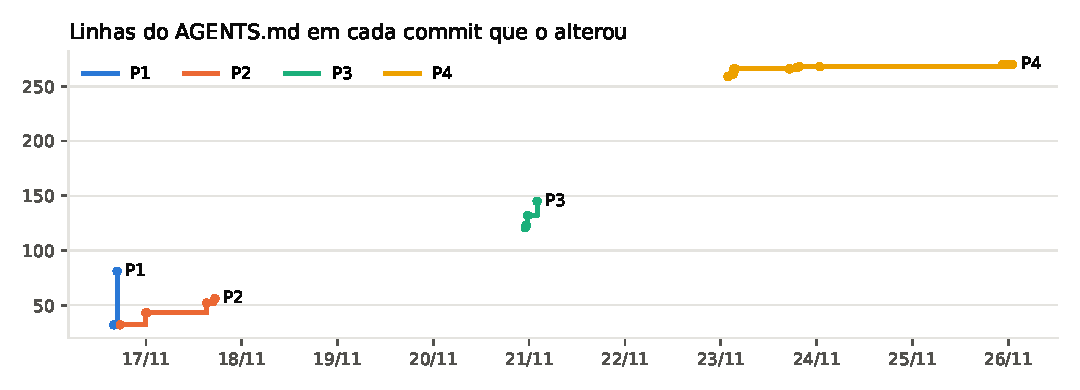
\includegraphics[width=\linewidth]{gerado/fig_agents_md.pdf}
\caption{Tamanho do \texttt{AGENTS.md} em cada commit que o alterou (todas as branches). Em
\Pum{} e \Pdois{} foi pequeno, tardio e centrado em git; em \Pquatro{} nasceu completo e mudou
pouco de tamanho, mas mudou muitas vezes de conteúdo.}
\label{fig:agents}
\end{figure}

A evolução tem três fases. Em \Pum{} e \Pdois{} as instruções eram \emph{reativas}: nasciam
depois de um problema (o commit sem corpo em \Pdois{}, a reorganização em \Pum{}) e tratavam de git.
Em \Ptres{} passaram a ser \emph{metodológicas} (âmbito por fase, regras que não se quebram). Em
\Pquatro{} tornaram-se \emph{um contrato de trabalho completo} desde o primeiro commit, incluindo
as regras de interação que faltavam (explicar comandos antes, pedir autorização, push só a
pedido). Duas lições laterais: copiar um \texttt{AGENTS.md} antigo sem o rever custa horas
(\Pdois); e uma regra que precisa de cinco exceções em duas horas (as cores em \Pquatro) é uma
regra mal desenhada.

\subsection{Comunicação entre utilizador e agente}

\begin{table}[H]
\centering\small
\caption{Como o utilizador comunicava com o agente.}
\begin{tabularx}{\linewidth}{@{}>{\raggedright\arraybackslash}p{2.7cm}LLLL@{}}
\toprule
 & \Pum & \Pdois & \Ptres & \Pquatro \\
\midrule
Canal principal & proposta, revisões, \emph{spec}/\emph{plan} & prompts e documentos-plano externos & AGENTS.md + plano com decisões D1--D18 & AGENTS.md, docs/00--01, decisões REV e D1--D8 \\
Antes de agir & — & — & perguntar em vez de inventar & explicar comando, efeitos; esperar pelo sim \\
Depois de agir & corpo do commit & corpo do commit com «Verificação» & commit O quê/\dots/Pendente & resumo + commit + PROGRESS + handoff \\
Decisões do utilizador & implícitas & no plano & D1--D18 & REV com citação; autorizações em JSON \\
Língua & PT e EN misturados & PT; AGENTS em EN & PT-PT & PT-PT \\
\bottomrule
\end{tabularx}
\end{table}

O padrão que funcionou em \Pquatro{} foi \emph{separar três coisas}: a decisão do utilizador
(registada com ID), a autorização (escrita, com âmbito) e a execução (feita e validada pelo
agente). As tabelas de decisões com recomendação e alternativa (D1--D8) tornaram as perguntas
rápidas de responder. Nas tentativas anteriores, o utilizador queixava-se de que os agentes
ignoravam regras e de explicações pouco claras; o modelo de commit de \Ptres{} e a obrigação de
explicar antes de executar em \Pquatro{} atacaram diretamente essas queixas.

\subsection{Memória e continuidade}

\begin{table}[H]
\centering\small
\caption{Mecanismos para guardar estado e raciocínio entre sessões.}
\begin{tabularx}{\linewidth}{@{}>{\raggedright\arraybackslash}p{2.7cm}LLLL@{}}
\toprule
 & \Pum & \Pdois & \Ptres & \Pquatro \\
\midrule
Estado vivo & planos com checkboxes (0 de 78 marcadas) & plano vivo + auditorias & plano com estado por passo & PROGRESS (topo vivo) \\
Decisões & — & dispersas & D1--D18 no plano & REV-001--083 + «Decisões vigentes» \\
Passagem entre sessões & — & — & mensagens de commit & handoff.md com hora e última validação \\
Experiências & — & CSV EXP-001--009 & registo EXP & resultados + macros geradas \\
Problema principal & docs fora do git & estado em 4--5 sítios & sem estado da conversa & redundância e custo \\
\bottomrule
\end{tabularx}
\end{table}

A peça decisiva foi o \texttt{handoff.md}: um ficheiro curto, reescrito de raiz, que diz onde se
está, o que ler primeiro, o que foi validado e \emph{a que horas}, e o que falhou. Foi o que
permitiu mudar de conversa e de modelo quatro vezes sem perder o fio. O preço foi a redundância: o
mesmo facto escrito no \texttt{REVISION\_LOG}, no \texttt{PROGRESS}, no \texttt{handoff} e por
vezes no \texttt{README} e em \texttt{docs/00}.

\subsection{Segurança}

\begin{table}[H]
\centering\small
\caption{Segurança dos dados, do git e do ambiente.}
\begin{tabularx}{\linewidth}{@{}>{\raggedright\arraybackslash}p{2.7cm}LLLL@{}}
\toprule
 & \Pum & \Pdois & \Ptres & \Pquatro \\
\midrule
Divisão & por navio → por viagem & por viagem, seed 42 & por viagem, seed 42 & por viagem, seed 42, manifesto versionado \\
Uso de val./teste em desenvolvimento & EDA antes da divisão & leitura exploratória & percentis por conjunto & proibido; autorização escrita + registo \\
Dados no git & sim (≈202~MB) & não & não & não (só o manifesto) \\
Push & regra tardia (sem force) & «nunca force» & sem regra & só a pedido explícito \\
Reutilização do conjunto final & — & — & — & 3 usos, registados \\
\bottomrule
\end{tabularx}
\end{table}

A segurança melhorou de forma monótona, e o salto maior foi passar de \emph{intenções}
(«não usar o teste») para \emph{mecanismos} (código que recusa abrir sem autorização, testes
desse código, registo de acessos). Mesmo assim, o mecanismo de \Pquatro{} só protegia contra o
agente: não impediu o próprio utilizador de reutilizar o conjunto final, nem de retirar do resumo
a ressalva de que o resultado do filtro não era uma medição independente (REV-068). A
transparência dependeu do registo, não do bloqueio.

\subsection{Fiabilidade e reprodutibilidade}

\Pum{} tinha poucos testes mas bons; \Pdois{} e \Ptres{} trocaram testes por \texttt{assert} em
scripts e verificação manual nos commits; \Pquatro{} voltou aos testes sintéticos a sério e
juntou-lhes a regra de que \emph{nenhum número do relatório pode vir de um cálculo informal do
agente}. Esta regra, com as macros geradas, é provavelmente a melhor defesa contra a tendência dos
agentes para afirmar resultados sem evidência. A outra metade da fiabilidade foi a honestidade
sobre o que foi validado: o handoff de \Pquatro{} diz o que foi verificado, quando, e o que
\emph{não} foi repetido.

\subsection{Produtividade: «muito por pouco»}

\begin{figure}[H]
\centering
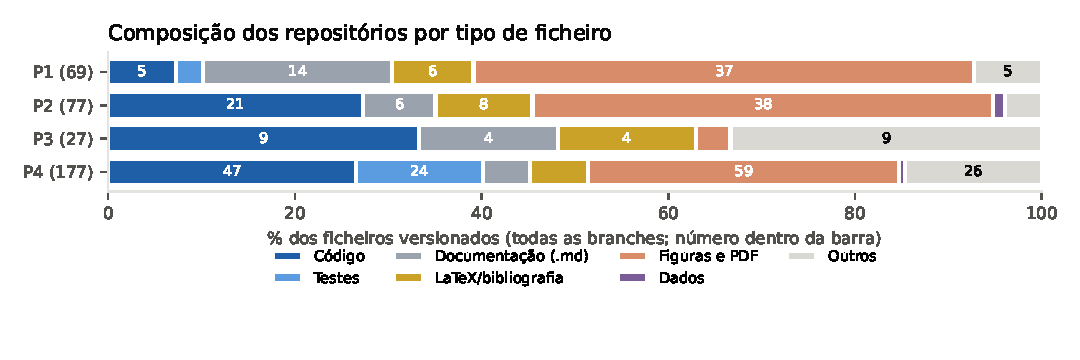
\includegraphics[width=\linewidth]{gerado/fig_composicao.pdf}
\caption{Composição dos repositórios por tipo de ficheiro (união das branches; «Figuras e PDF»
inclui bibliografia e PDFs da proposta).}
\label{fig:composicao}
\end{figure}

A queixa central do utilizador aparece nas quatro tentativas com formas diferentes:

\begin{itemize}
  \item \Pum: \textbf{exploração sem fim} — 48\,\% do código em figuras, nenhum modelo.
  \item \Pdois: \textbf{documentação e sincronização} — auditorias, plano de 1\,475 linhas, 10
        versões do PDF, estado duplicado; modelo não treinado.
  \item \Ptres: \textbf{sobre-engenharia fora do âmbito} — HMM de raiz e BiGRU em vez da CNN.
  \item \Pquatro: \textbf{contabilidade e relatório} — 25\,\% dos commits só de registo, 3\,839
        linhas de código de figuras e diagnóstico contra 1\,921 de núcleo, 10 revisões
        cosméticas.
\end{itemize}

\deducao{} Os agentes tendem a preencher o espaço que lhes é dado com trabalho \emph{visível}
(figuras, documentos, registos) quando falta um critério explícito de progresso. O que reduziu o
problema em \Pquatro{} foram os marcos executáveis com critério de fecho; o que o manteve foi a
regra de atualizar registos em \emph{cada} interação. Foi por isto que o utilizador experimentou
a skill \emph{Ponytail} (modo «mínima alteração»), que não deixou vestígios no repositório.

\subsection{Estrutura do repositório}

\Pum{} mudou a raiz duas vezes e teve três versões da proposta; \Pdois{} teve três cópias da
organização (em \texttt{main} e em dois ramos-\emph{snapshot}); \Ptres{} e \Pquatro{} foram limpos.
A diferença está em ter decidido a estrutura no primeiro dia e em usar \emph{tags} (não ramos)
para guardar versões, como \Pquatro{} fez com \texttt{proposta-pt-v1} e \texttt{docs-historico-v1}.

%% =====================================================================
\section{Balanço: o que correu bem e o que correu mal}\label{sec:balanco}

\subsection{O que correu bem (e deve repetir-se)}
\begin{enumerate}
  \item \textbf{Regras completas desde o primeiro commit} (\Pquatro), em vez de regras reativas.
  \item \textbf{Marcos executáveis} com critério de fecho e âmbito fechado por fase (\Ptres, \Pquatro).
  \item \textbf{Handoff com hora e última validação} (\Pquatro): continuidade entre conversas e modelos.
  \item \textbf{Decisões com ID} e \textbf{perguntas em tabela} com recomendação (\Pquatro).
  \item \textbf{Isolamento auditável} dos dados reservados: manifesto, autorização escrita antes
        de abrir, registo de acessos, testes do mecanismo (\Pquatro).
  \item \textbf{Números gerados por código} até ao LaTeX (\Pquatro).
  \item \textbf{Testes sintéticos} desde o primeiro dia (\Pum{} no conversor, \Pquatro{} em tudo).
  \item \textbf{Modelo de commit} O quê / Porquê / Validação / Pendente (\Ptres, \Pquatro).
  \item \textbf{Push só a pedido} e nunca por subagentes (\Pquatro).
  \item \textbf{Revisão independente só de leitura} antes da medição final e do relatório (\Pquatro).
  \item \textbf{Plano externo} preparado com um LLM de chat e entregue ao agente (\Pdois, \Pquatro).
\end{enumerate}

\subsection{O que correu mal no início}
\begin{enumerate}
  \item Instruções tardias e só sobre git (\Pum); instruções copiadas desatualizadas (\Pdois).
  \item Várias ferramentas em paralelo sem registo comum (\Pum).
  \item Exploração e figuras sem pergunta nem critério de paragem (\Pum).
  \item Dados e bibliografia no git; \texttt{docs/} fora do git (\Pum).
  \item Contacto exploratório com validação e teste (\Pum, \Pdois, \Ptres).
  \item Ramos usados como \emph{snapshots}; estrutura mudada de raiz (\Pum, \Pdois).
  \item Estado duplicado em muitos documentos e relatórios de estado otimistas (\Pdois).
  \item Modelo e âmbito desalinhados com o enunciado (\Ptres).
\end{enumerate}

\subsection{O que ainda correu mal em \Pquatro}
\begin{enumerate}
  \item \textbf{Contabilidade excessiva}: atualização obrigatória de dois registos em cada
        interação (REV-010); commits só para registar pushes, horas ou vigilantes; o
        \texttt{PROGRESS} e o \texttt{REVISION\_LOG} pesam quase tanto como o código.
  \item \textbf{Regra das cores rígida}: cinco exceções e quatro edições ao AGENTS.md em duas
        horas; a paleta deixou de ser mantida depois da REV-022.
  \item \textbf{Conjunto final reutilizado} três vezes por decisão do utilizador, e uma ressalva
        retirada do resumo; ficou registado, mas é um risco de integridade.
  \item \textbf{Código de relatório maior que o núcleo} e figuras órfãs.
  \item \textbf{AGENTS.md longo} (\mQuatroAgentsLinhas{} linhas) e ainda escrito para várias
        ferramentas depois de o Claude Code ter sido escolhido na primeira hora.
  \item \textbf{Uma revisão por ajuste cosmético} na fase de paginação do relatório.
\end{enumerate}

%% =====================================================================
\section{Lições para o próximo projeto}\label{sec:licoes}

\begin{licao}[1. Primeiro um resultado ponta a ponta, depois a exploração]
Definir o marco 2 como «dados → modelo simples → métrica» e não aceitar figuras ou estatísticas
que nenhuma decisão use. Cada exploração tem pergunta e critério de paragem escritos antes.
\end{licao}

\begin{licao}[2. As regras certas no primeiro commit, curtas]
Um \texttt{AGENTS.md} de cerca de 100 linhas, com âmbito, comunicação, dados, números, testes,
git e continuidade. Uma ponte de 3--5 linhas por ferramenta. Rever, não copiar, o do projeto
anterior.
\end{licao}

\begin{licao}[3. Separar decisão, autorização e execução]
Decisões do utilizador com ID e data, num só sítio. Autorizações escritas, com âmbito, antes de
qualquer ação sensível. O agente executa e prova o que fez.
\end{licao}

\begin{licao}[4. Mecanismos, não intenções, para o que não pode falhar]
Isolamento de dados reservados por código testado e registo de acessos; push só a pedido;
números só de código versionado. E decidir antes o que acontece se o conjunto final for
reutilizado (proibido, ou declarado no resumo).
\end{licao}

\begin{licao}[5. Continuidade leve]
Um \texttt{handoff.md} curto, reescrito no fim de cada \emph{sessão} (não de cada mensagem), com
hora lida com \texttt{date}. Um \texttt{PROGRESS.md} com topo vivo e registo cronológico. IDs de
revisão só para decisões metodológicas. Nada de commits só para registar horas ou pushes. As
cores no LaTeX podem ser substituídas por \texttt{latexdiff} entre \emph{tags}.
\end{licao}

\begin{licao}[6. Uma ferramenta principal, delegação com contrato]
Escolher uma ferramenta de agente por projeto. Delegar a subagentes ou a outras ferramentas só
tarefas com contrato fechado, passar-lhes as regras e rever a evidência. Uma revisão
independente só de leitura antes de cada entrega.
\end{licao}

\begin{licao}[7. Estrutura decidida no primeiro dia]
Pastas finais desde o início, dados e bibliografia fora do git, versões guardadas em
\emph{tags}, código de relatório separado do núcleo.
\end{licao}

%% =====================================================================
\section{Kit de arranque}\label{sec:kit}

A pasta \texttt{investigacao\_agentes/kit/} contém quatro ficheiros prontos a copiar para um
projeto novo, reproduzidos nos anexos:

\begin{itemize}
  \item \texttt{AGENTS\_modelo.md} (Anexo~\ref{an:agents}): as regras destiladas, em cerca de 100 linhas.
  \item \texttt{handoff\_modelo.md} (Anexo~\ref{an:handoff}): a passagem de testemunho entre sessões.
  \item \texttt{PROGRESS\_modelo.md} (Anexo~\ref{an:progress}): estado vivo, decisões e registo,
        juntando o que em \Pquatro{} estava em dois ficheiros.
  \item \texttt{checklist\_arranque.md} (Anexo~\ref{an:checklist}): o que fazer antes da primeira
        sessão, na primeira sessão, em cada sessão e antes de entregar.
\end{itemize}

A mensagem para abrir cada conversa mantém-se a de \Pquatro: «Lê o AGENTS.md e o handoff.md e
diz-me o ponto de situação.»

%% =====================================================================
\section{Limitações e ameaças à validade}\label{sec:validade}

\begin{itemize}
  \item \textbf{Sem as conversas.} O que o utilizador disse ao agente só se vê pelos efeitos no
        repositório; motivos de recomeço e frustrações vêm do utilizador ou são deduções.
  \item \textbf{Ferramentas deduzidas.} Os \emph{trailers} só existem quando a ferramenta os
        acrescenta; a ausência de vestígios não prova que uma ferramenta não foi usada.
  \item \textbf{Métricas de volume.} Linhas e commits medem esforço visível, não valor. A
        composição por tipo de ficheiro conta ficheiros, não tamanho.
  \item \textbf{Aprendizagem acumulada.} \Pquatro{} beneficiou de tudo o que se aprendeu antes,
        incluindo o conhecimento do problema; nem toda a melhoria se deve ao fluxo de trabalho
        ou à ferramenta.
  \item \textbf{Análise feita com o mesmo tipo de agente.} Os relatórios por repositório foram
        escritos por subagentes; as afirmações centrais foram verificadas por amostragem, não
        todas.
\end{itemize}

%% =====================================================================
\section*{Declaração de uso de inteligência artificial}
\addcontentsline{toc}{section}{Declaração de uso de inteligência artificial}

Este documento foi gerado automaticamente com inteligência artificial, coerentemente com o
fluxo de trabalho com agentes usado em todo o projeto. Foi produzido pelo Claude Code (modelo
Claude Opus 5.5, da Anthropic) a pedido e sob a orientação de Dinis Rosa, que definiu o âmbito,
as fontes, o público e o formato através de perguntas e respostas. A análise dos repositórios
foi feita por quatro subagentes (Claude Opus), um por repositório, só em modo de leitura; o
agente coordenador integrou os relatórios, verificou por amostragem as afirmações centrais,
escreveu o script de métricas, os modelos do kit e este texto. As perceções pessoais (o que
frustrou, o que funcionou, porque se recomeçou) são do autor; o resto deve ser lido como uma
análise assistida por IA, com as limitações da Secção~\ref{sec:validade}.

%% =====================================================================
\newpage
\appendix
\section{Métricas e como reproduzi-las}\label{an:metricas}

Para regenerar \texttt{gerado/} (a partir da raiz do repositório, com clones dos quatro
repositórios):

\begin{lstlisting}
git clone https://github.com/DinisRosa/IACH-AIS-Project.git    /tmp/r/P1
git clone https://github.com/DinisRosa/IACH-AIS-Project_2.git  /tmp/r/P2
git clone https://github.com/DinisRosa/IACH-AIS-Project_3.git  /tmp/r/P3
git clone https://github.com/DinisRosa/IACH-AIS-Project_4.git  /tmp/r/P4
iach-ais-venv-4/bin/python investigacao_agentes/scripts/metricas_git.py \
    P1=/tmp/r/P1 P2=/tmp/r/P2 P3=/tmp/r/P3 P4=/tmp/r/P4
\end{lstlisting}

\begin{table}[H]
\centering\small
\caption{Todas as métricas usadas (as de \Pquatro{} medidas no commit \texttt{0337bfa}).}
\begin{tabularx}{\linewidth}{@{}Lrrrr@{}}
\toprule
Métrica & \Pum & \Pdois & \Ptres & \Pquatro \\
\midrule
Commits (todas as branches) & \mUmCommits & \mDoisCommits & \mTresCommits & \mQuatroCommits \\
Dias com commits & \mUmDias & \mDoisDias & \mTresDias & \mQuatroDias \\
Branches remotas & \mUmBranches & \mDoisBranches & \mTresBranches & \mQuatroBranches \\
Ficheiros versionados (união das branches) & \mUmFicheiros & \mDoisFicheiros & \mTresFicheiros & \mQuatroFicheiros \\
Linhas Python sem testes (branch por defeito) & \mUmLinhasPy & \mDoisLinhasPy & \mTresLinhasPy & \mQuatroLinhasPy \\
Linhas de testes & \mUmLinhasTestes & \mDoisLinhasTestes & \mTresLinhasTestes & \mQuatroLinhasTestes \\
Funções \texttt{def test\_} & \mUmFuncTestes & \mDoisFuncTestes & \mTresFuncTestes & \mQuatroFuncTestes \\
Linhas Markdown & \mUmLinhasMd & \mDoisLinhasMd & \mTresLinhasMd & \mQuatroLinhasMd \\
Versões do AGENTS.md & \mUmAgentsVersoes & \mDoisAgentsVersoes & \mTresAgentsVersoes & \mQuatroAgentsVersoes \\
Linhas do AGENTS.md (primeira / última) & \mUmAgentsPrimeiro{} / \mUmAgentsLinhas & \mDoisAgentsPrimeiro{} / \mDoisAgentsLinhas & \mTresAgentsPrimeiro{} / \mTresAgentsLinhas & \mQuatroAgentsPrimeiro{} / \mQuatroAgentsLinhas \\
Commits com \emph{trailer} de coautoria & \mUmCoAutor & \mDoisCoAutor & \mTresCoAutor & \mQuatroCoAutor \\
Commits só de registo (PROGRESS, REVISION\_LOG, handoff, README) & \mUmRegisto & \mDoisRegisto & \mTresRegisto & \mQuatroRegisto \\
Commits só com Markdown & \mUmSoMd & \mDoisSoMd & \mTresSoMd & \mQuatroSoMd \\
Commits que citam um ID REV & \mUmComRev & \mDoisComRev & \mTresComRev & \mQuatroComRev \\
\bottomrule
\end{tabularx}
\end{table}

\section{Modelo de AGENTS.md}\label{an:agents}
\lstinputlisting{kit/AGENTS_modelo.md}

\section{Modelo de handoff.md}\label{an:handoff}
\lstinputlisting{kit/handoff_modelo.md}

\section{Modelo de PROGRESS.md}\label{an:progress}
\lstinputlisting{kit/PROGRESS_modelo.md}

\section{Checklist de arranque}\label{an:checklist}
\lstinputlisting{kit/checklist_arranque.md}

\end{document}
